% !TEX root = prime_factors.tex

\section{\en Finding LCM and HCF from prime factors \cy Canfod LlCLl a FfCM o rhifau cysefin}
\label{sec:finding-hcf-and-lcm-from-prime-factors}

\en Sometimes you are given numbers expressed as a product of prime factors. For example, 
\cy Weithiau, byddi'n cael rhifau wedi eu mynegi fel lluoswm o ffactorau cysefin. Er enghraifft, 
\bi $8 = 2^3$ \en and \cy ac $90 = 2 \times 3^2 \times 5$.

\en If you want to find the LCM and HCF in an exam, we can use prime factor form to simplify the process.
\cy Os wyt ti eisiau canfod y LlCLl a'r FfCM mewn arholiad, gallwn ddefnyddio dull y ffactorau cysefin i symleiddio'r broses.

\begin{example}
Find the LCM and HCF of 18 and 30.
Canfydda LlCLl a FfCM 18 a 30.

\begin{solution}

Firstly, we write the numbers as a product of prime factors.
Yn gyntaf, rydyn ni'n ysgrifennu'r rhifau fel lluoswm o ffactorau cysefin.

\begin{align*}
18 	& = 2 \times 3 \times 3 = 2 \times 32 \\
30	& = 2 \times 3 \times 5
\end{align*}

Then we create a Venn diagram for the factors:
Yna rydyn ni'n creu diagram Venn ar gyfer y ffactorau:

\begin{figure}[H]
\centering
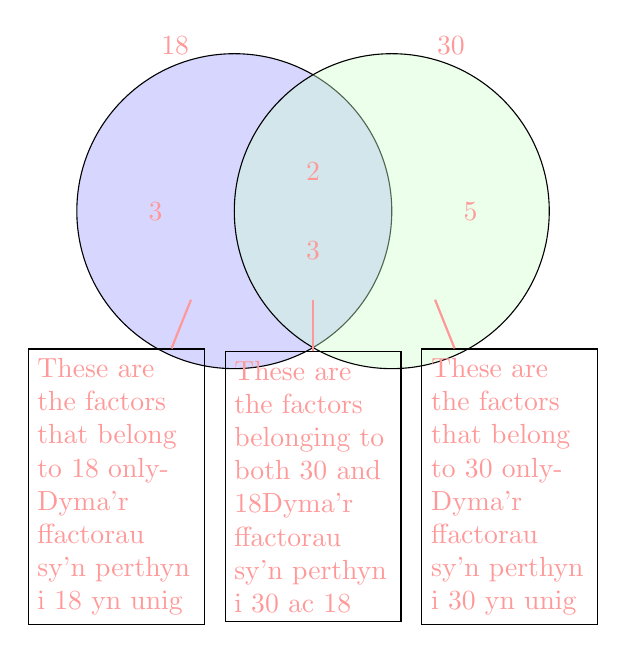
\begin{tikzpicture}
\begin{scope}[fill opacity=0.4]
	\tikzset{text opacity=1}
    \draw[fill=blue!40] (-1.0,0) circle (2);
    \draw[fill=green!20] (+1.0,0) circle (2);
    \node at (-1.75,2.1) {18};
    \node at (+1.75,2.1) {30};
    \node at (-2,0) {3};
    \node at (+2,0) {5};
    \node at (0,+0.5) {2};
    \node at (0,-0.5) {3};
    \node[draw, text width=2cm] at (-2.5,-3.5) (A)
    {\bil{These are the factors that belong to 18 only}{Dyma'r\\ ffactorau sy'n perthyn i 18 yn unig}};
    \node[draw, text width=2cm] at ( 0.0,-3.5) (B)
    {\bil{These are the factors belonging to both 30 and 18}{Dyma'r\\ ffactorau sy'n perthyn i 30 ac 18}};
    \node[draw, text width=2cm] at (+2.5,-3.5) (C)
    {\bil{These are the factors that belong to 30 only}{Dyma'r\\ ffactorau sy'n perthyn i 30 yn unig}};
	\node at (-1.5,-1) (A2) {};
    \node at ( 0.0,-1) (B2) {};
    \node at (+1.5,-1) (C2) {};
	\tikzset{color=red!40}
	\draw [red!40,thick] (A)--(A2);
	\draw [red!40,thick] (B)--(B2);
	\draw [red!40,thick] (C)--(C2);
\end{scope}
\end{tikzpicture}
\end{figure}

\en
Once we have the Venn diagram, finding the LCM is simply a matter of multiplying all the numbers in the Venn diagram together:
\cy
Unwaith mae gennyn ni'r diagram Venn, yn syml, gallwn luosi'r holl rifau yn y diagram Venn i ganfod y LlCLl:
\bi
\[
\text{\bil{LCM}{LlCLl}} = 3 \times 2 \times 3 \times 5 = 90.
\]

\en To find the HCF we multiply the numbers in the overlapping quadrant together:
\cy I ganfod y FfCM, rydyn ni'n lluosi'r rhifau yn y rhan sy'n gorgyffwrdd gyda'i gilydd:
\bi
\[
\text{\bil{HCF}{FfCM}} = 2 \times 3 = 6.
\]
\en
It is important to note that when you have two numbers, and are asked to find the HCF and LCM, the LCM will be the larger of the two numbers.
\cy
Mae'n bwysig i ni nodi hyn: pan fydd gen ti ddau rif, a bod gofyn i ti ganfod y FfCM a'r LlCLl, y LlCLl fydd y mwyaf o'r ddau rif.

\end{solution}
\end{example}

\begin{example}
\en Find the LCM and HCF of 50 and 16.
\cy Canfydda LlCLl a FfCM 50 ac 16.

\begin{solution}
\en Firstly, we write the numbers in prime factor form:
\cy Yn gyntaf, rydyn ni'n ysgrifennu'r rhifau ar ffurf ffactorau cysefin:
\bi
\begin{align*}
50	& = 2 \times 5 \times 5 = 2 \times 52 \\
16 	& = 2 \times 2 \times 2 \times 2 = 24
\end{align*}

\en We then draw the Venn diagram:
\cy Yna rydyn ni'n llunio'r diagram Venn:

\begin{figure}[H]
\centering
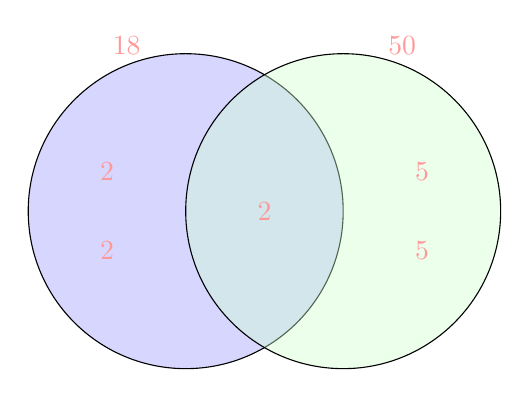
\begin{tikzpicture}
\begin{scope}[fill opacity=0.4]
	\tikzset{text opacity=1}
    \draw[fill=blue!40] (-1.0,0) circle (2);
    \draw[fill=green!20] (+1.0,0) circle (2);
    \node at (-1.75,2.1) {18};
    \node at (+1.75,2.1) {50};
    \node at (-2,+0.5) {2};
    \node at (-2,-0.5) {2};
    \node at (0,0) {2};
    \node at (+2,-0.5) {5};
    \node at (+2,+0.5) {5};
\end{scope}
\end{tikzpicture}
\end{figure}

\en 
As both numbers have 2 as a factor, this goes in the middle. The remaining factors go in their respective circles.
\cy
Gan fod 2 yn ffactor i'r ddau rif, mae hwn yn mynd yn y canol. Mae'r ffactorau sydd dros ben yn mynd yn eu cylchoedd perthnasol.

\en
The LCM is found by multiplying all of the numbers in the Venn diagram together. As there are four 2s and two 5s:
\cy
Cawn y LlCLl drwy luosi'r holl rifau yn y diagram Venn gyda'i gilydd. Gan fod yna bedwar rhif 2 a dau rif 5:
\bi
\[
\text{\bil{LCM}{FfCM}}= 2 \times 2 \times 2 \times 2 \times 5 \times 5 = 400
\]
\en
The HCF is found by multiplying together all of the numbers in the overlapping quadrant. As there is only one number present, HCF = 2.
\cy
Cawn y FfCM drwy luosi'r holl rifau sydd yn y rhan sy'n gorgyffwrdd gyda'i gilydd. Gan mai dim ond un rhif sydd yno: FfCM = 2.

\end{solution}
\end{example}

